\section{Volatility forecasting}
\label{sec:forecasting}

\subsection{Forecasting dataset and temporal split}

The forecasting experiment evaluates whether RMT and network features contain incremental information for realized volatility. The experiment is deliberately conservative. It uses PETR4, VALE3 and BBDC4 as target assets and compares network-augmented machine-learning models with strong econometric baselines. The data are split temporally: training covers 2006--2017, validation covers 2018--2020 and testing covers 2021--2025. This strict temporal split avoids random cross-sectional leakage across time and ensures that model selection is not based on future observations.

\subsection{GARCH persistence and econometric benchmarks}

The GARCH(1,1) estimates with Student-$t$ innovations confirm high volatility persistence. Table~\ref{tab:garch_params} reports $\omega$, $\alpha$, $\beta$ and $\alpha+\beta$. The persistence values are 0.9911 for PETR4, 0.9946 for VALE3 and 0.9828 for BBDC4. These high values explain why classical volatility benchmarks are difficult to outperform and are consistent with the slow ACF decay of absolute returns documented in Section~\ref{sec:stylized_correlation}.

\begin{table}
\centering
\caption{GARCH(1,1) persistence estimates for the forecasting assets.}
\label{tab:garch_params}
\begin{tabular}{lrrrr}
\toprule
Asset & $\omega$ & $\alpha$ & $\beta$ & $\alpha+\beta$ \\
\midrule
BBDC4 & 0.0729 & 0.0520 & 0.9308 & 0.9828 \\
PETR4 & 0.0780 & 0.0758 & 0.9153 & 0.9911 \\
VALE3 & 0.0417 & 0.0512 & 0.9434 & 0.9946 \\
\bottomrule
\end{tabular}
\end{table}
\FloatBarrier

\subsection{Machine-learning feature sets}

The machine-learning models use three nested feature sets in an ablation design. Set~A contains classical volatility features. Set~B adds market and RMT variables. Set~C adds MST and PMFG network variables. This nesting allows the paper to isolate whether network topology adds information beyond classical lagged-volatility persistence and broad market-mode features.

\subsection{Out-of-sample model comparison}

Figure~\ref{fig:forecast_comparison} summarizes out-of-sample QLIKE loss. Lower QLIKE is better. The figure uses the best feature set for each machine-learning model and horizon, avoiding ambiguous labels and making the comparison easier to interpret.

\begin{figure}
\centering
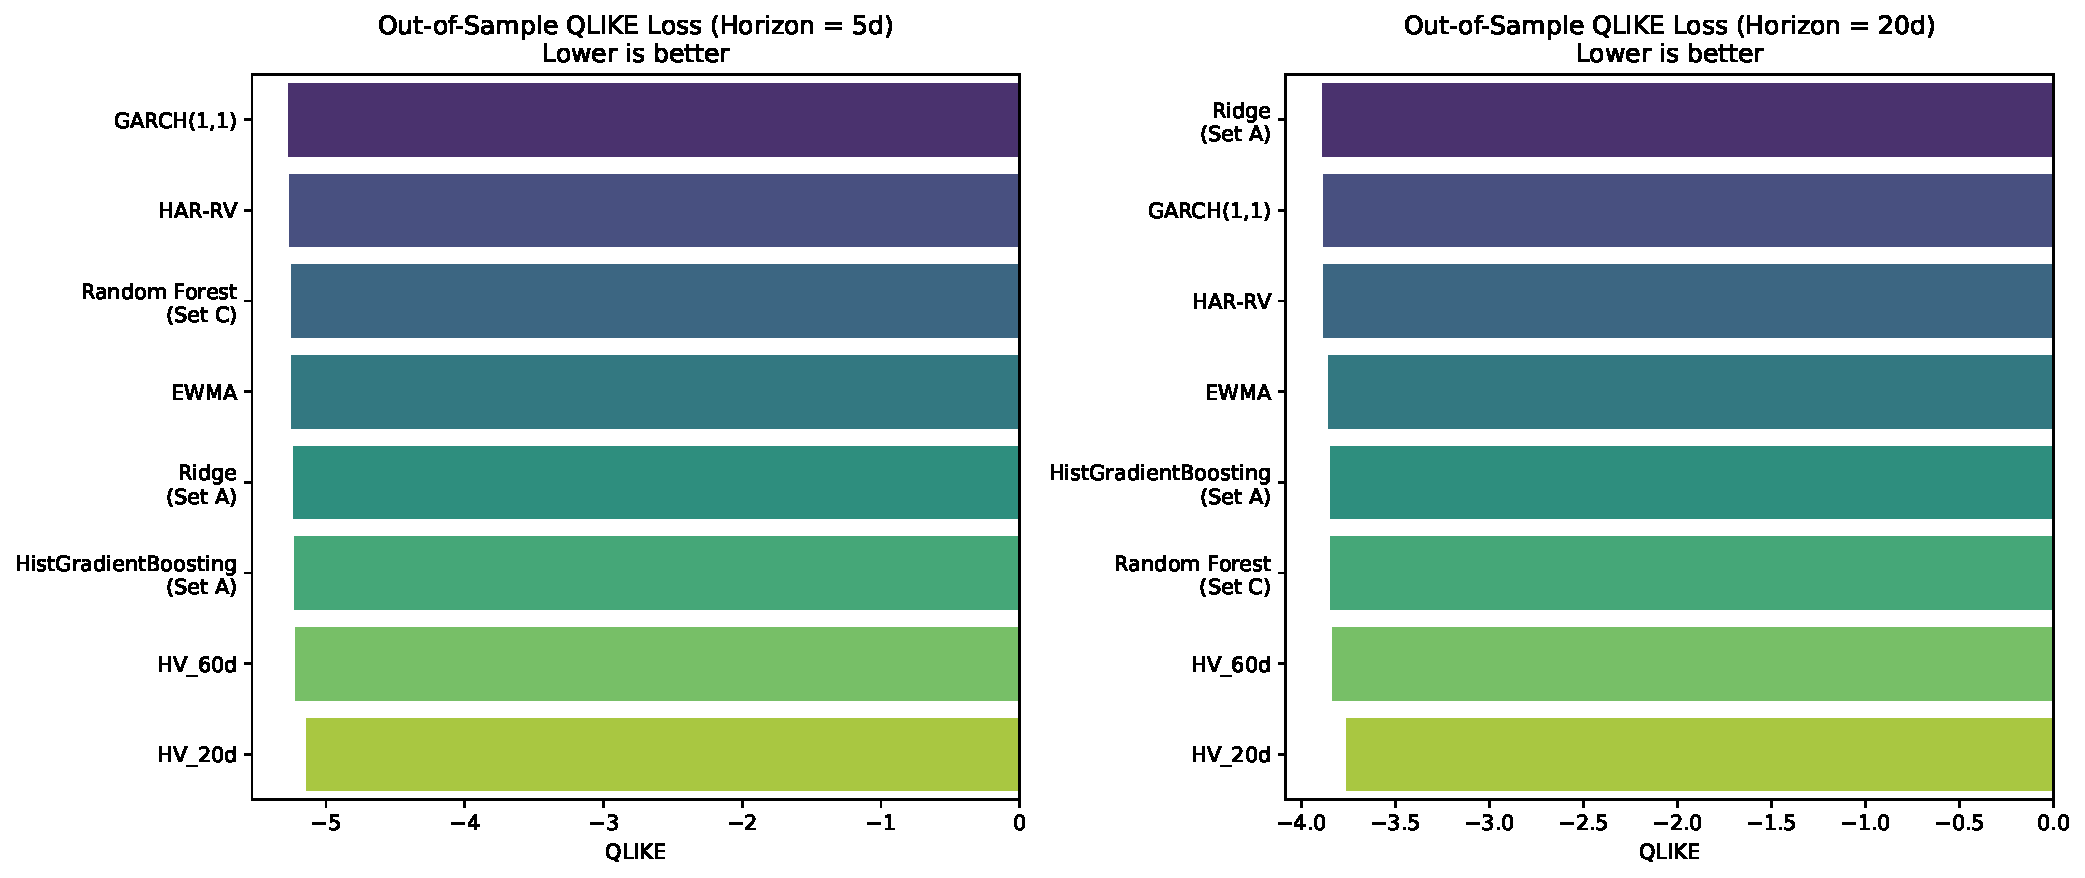
\includegraphics[width=\linewidth]{images/figure_16_volatility_forecast_model_comparison.pdf}
\caption{Volatility forecasting comparison for econometric and machine-learning models. Machine-learning labels show the best feature set selected for each model and horizon.}
\label{fig:forecast_comparison}
\end{figure}
\FloatBarrier

At the 5-day horizon, GARCH(1,1), HAR-RV and Random Forest are highly competitive. GARCH has average test QLIKE close to -5.27, HAR-RV is close to -5.26 and Random Forest with Set C is close to -5.25. The differences are small, which means the safe interpretation is not that machine learning dominates. Rather, the network-augmented model approaches strong classical benchmarks.

At the 20-day horizon, Ridge models with Set A or Set B compete strongly and slightly outperform GARCH in average QLIKE. Ridge Set A and Set B are close to -3.89, while GARCH is close to -3.88. Random Forest Set C remains competitive but does not dominate. This result suggests that longer-horizon volatility may be easier to forecast with stable linear shrinkage features, while nonlinear models require careful regularization and validation.

\begin{table}
\centering
\caption{Aggregated test-set forecasting comparison (2021--2025). Values are averaged across PETR4, VALE3 and BBDC4.}
\label{tab:forecast_comparison}
\resizebox{\linewidth}{!}{%
\begin{tabular}{llrrrrr}
\toprule
Horizon & Model & Feature set & MAE & RMSE & QLIKE & $R^2_{\mathrm{oos}}$ \\
\midrule
5 & GARCH(1,1) & Classical & 0.0156 & 0.0213 & $-5.27$ & 0.16 \\
5 & HAR-RV & Classical & 0.0148 & 0.0198 & $-5.26$ & 0.22 \\
5 & Random Forest & Set C (+Network) & 0.0151 & 0.0204 & $-5.25$ & 0.20 \\
5 & EWMA & Classical & 0.0153 & 0.0207 & $-5.25$ & 0.19 \\
20 & Ridge & Set A (Classical) & 0.0241 & 0.0328 & $-3.89$ & 0.39 \\
20 & Ridge & Set B (+Market/RMT) & 0.0242 & 0.0329 & $-3.89$ & 0.39 \\
20 & GARCH(1,1) & Classical & 0.0278 & 0.0381 & $-3.88$ & 0.23 \\
20 & HAR-RV & Classical & 0.0260 & 0.0356 & $-3.88$ & 0.28 \\
20 & Random Forest & Set C (+Network) & 0.0287 & 0.0393 & $-3.85$ & 0.17 \\
\bottomrule
\end{tabular}}
\end{table}
\FloatBarrier

\subsection{Realized vs predicted volatility diagnostics}

Aggregate metrics can hide important time-series behaviour. Figure~\ref{fig:realized_vs_predicted} compares realized 20-day volatility with GARCH and Random Forest forecasts for PETR4, VALE3 and BBDC4. This diagnostic is included in the body because it shows how models react to volatility regimes.

\begin{figure}
\centering
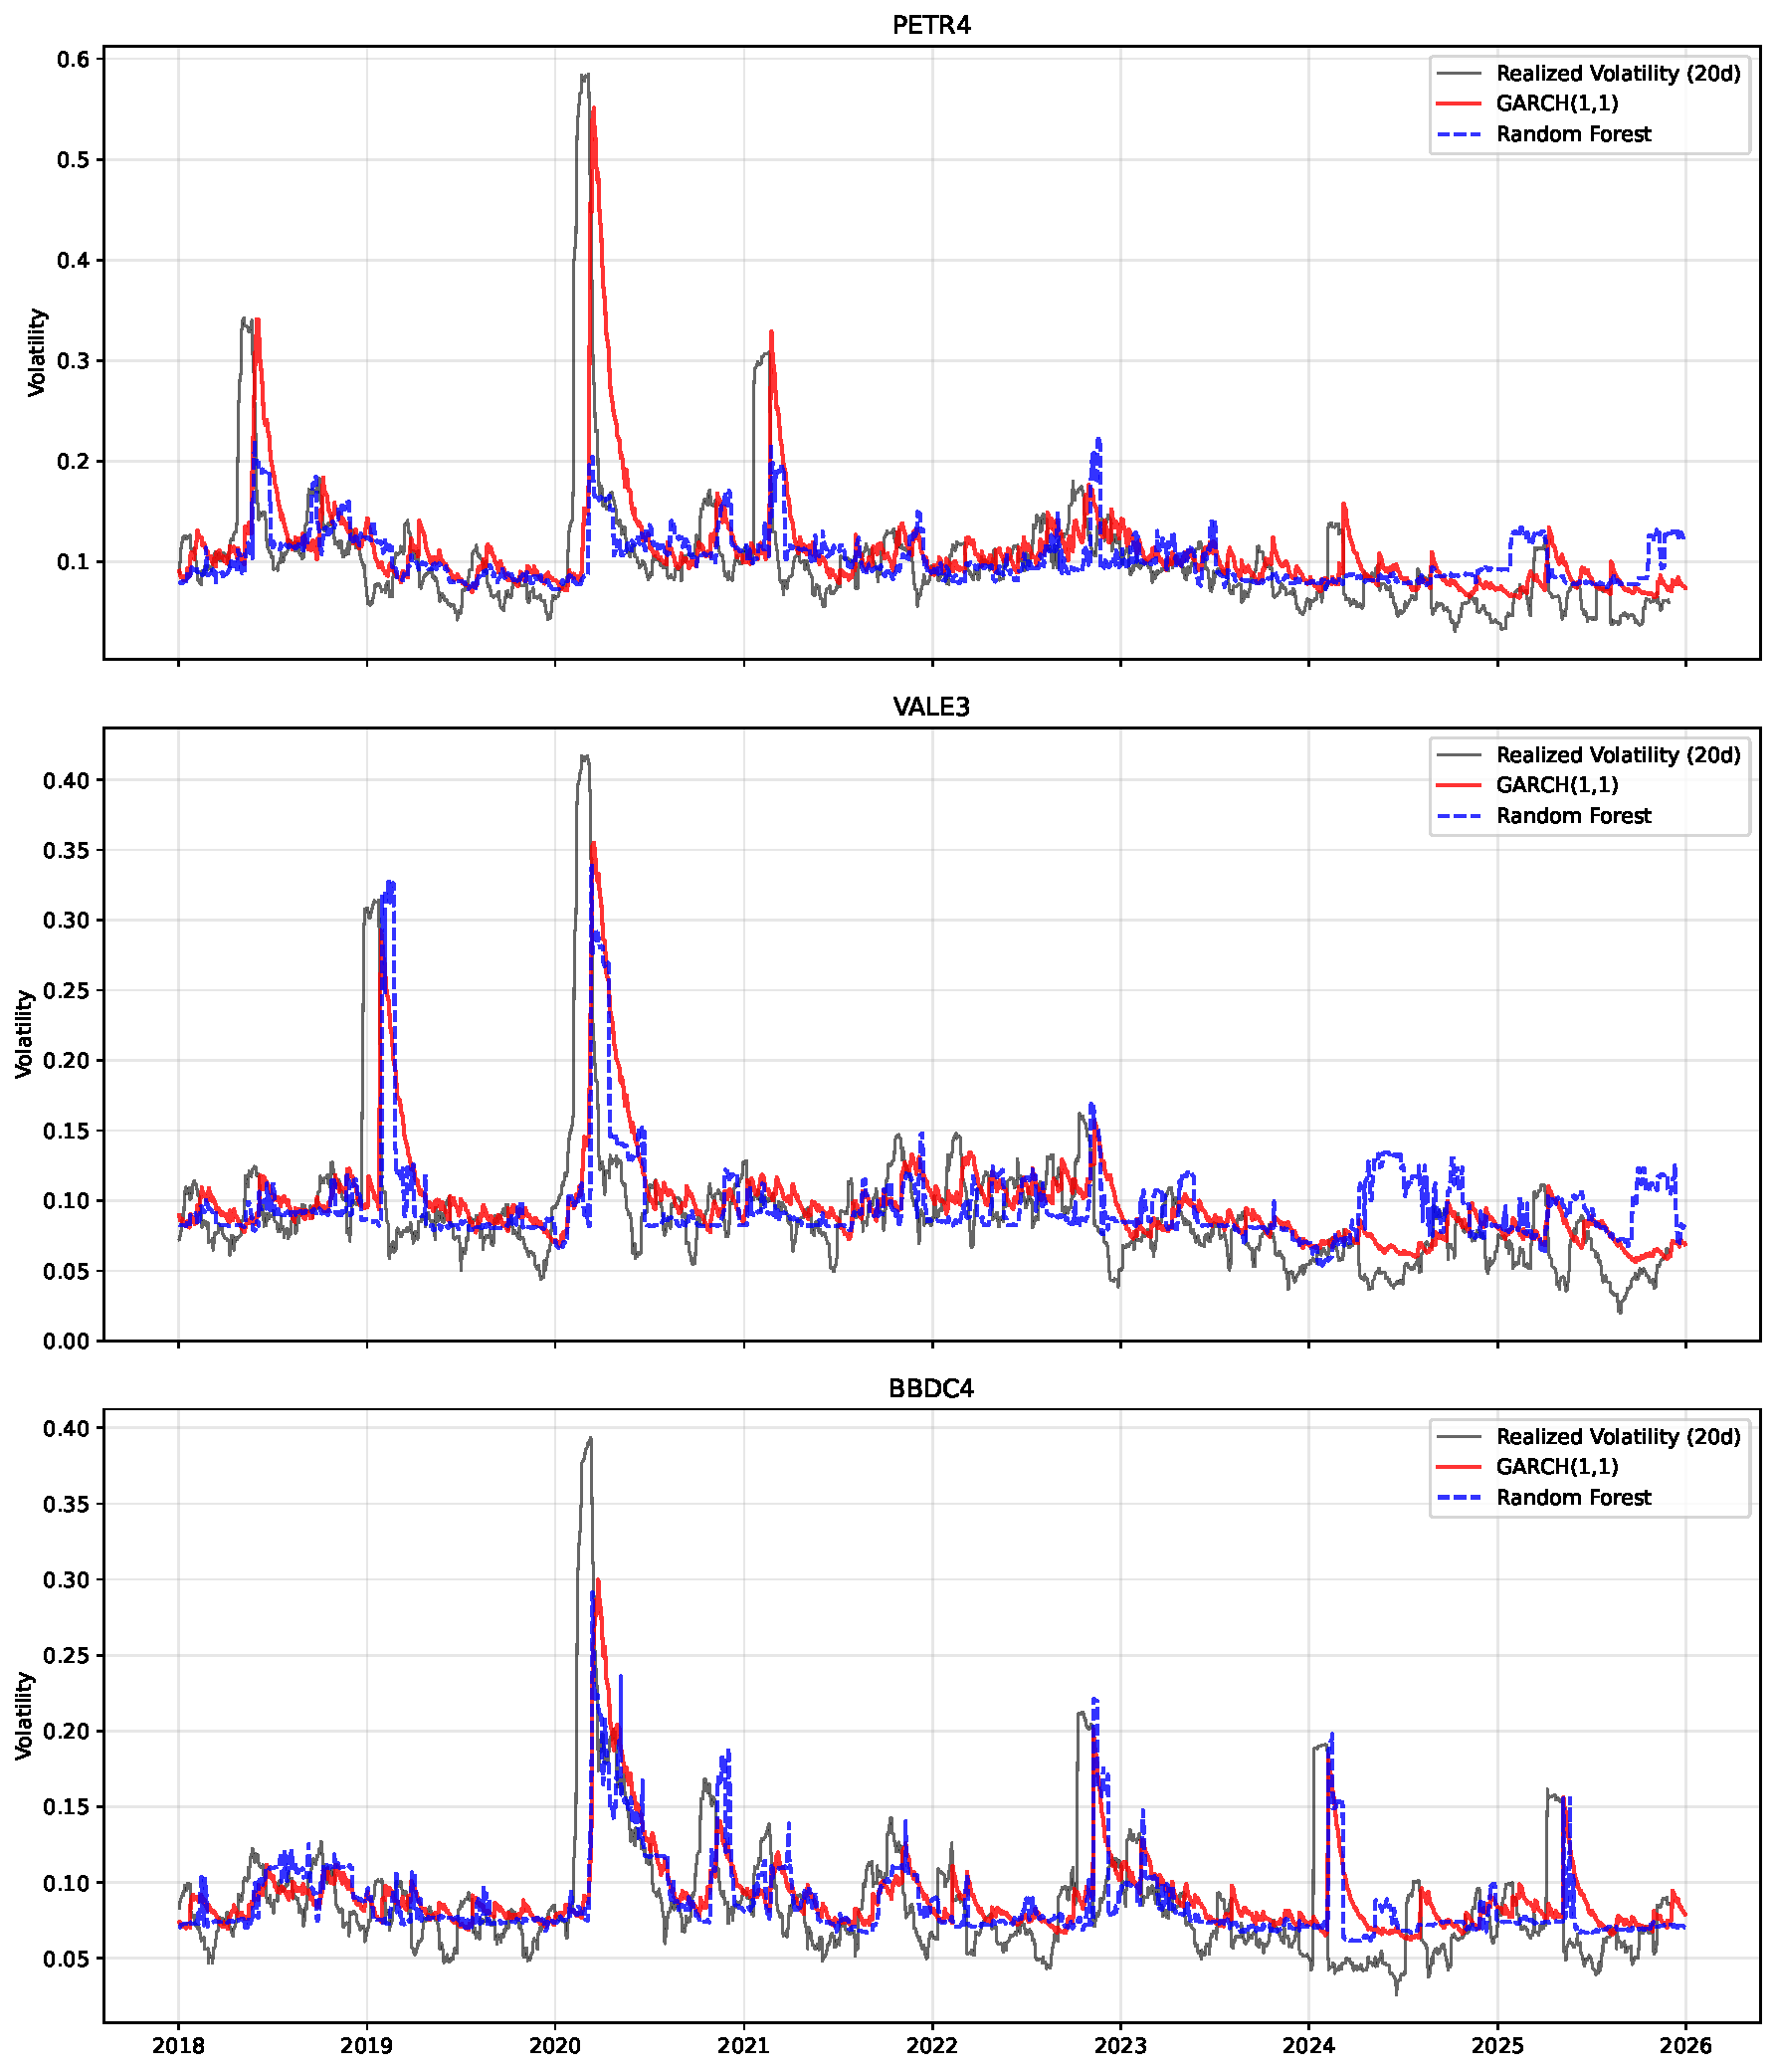
\includegraphics[width=0.95\linewidth]{images/figure_17_realized_vs_predicted_volatility.pdf}
\caption{Realized versus predicted 20-day volatility for selected models and assets. The plot illustrates regime tracking and forecast smoothness.}
\label{fig:realized_vs_predicted}
\end{figure}
\FloatBarrier

The diagnostic plots show that broad volatility regimes are captured, but extreme spikes remain difficult. GARCH reacts strongly to shock persistence, while Random Forest predictions can be smoother or more step-like depending on feature regimes. This behaviour is consistent with the aggregate results: nonlinear models can be competitive, but the dominant forecasting signal remains volatility persistence.

\subsection{Feature importance and network signal}

Feature importance provides a direct view of what the Random Forest uses. Figure~\ref{fig:feature_importance} shows that classical volatility features dominate the model. Rolling absolute returns, lagged realized volatility, rolling volatility and EWMA variables carry most of the importance.

\begin{figure}
\centering
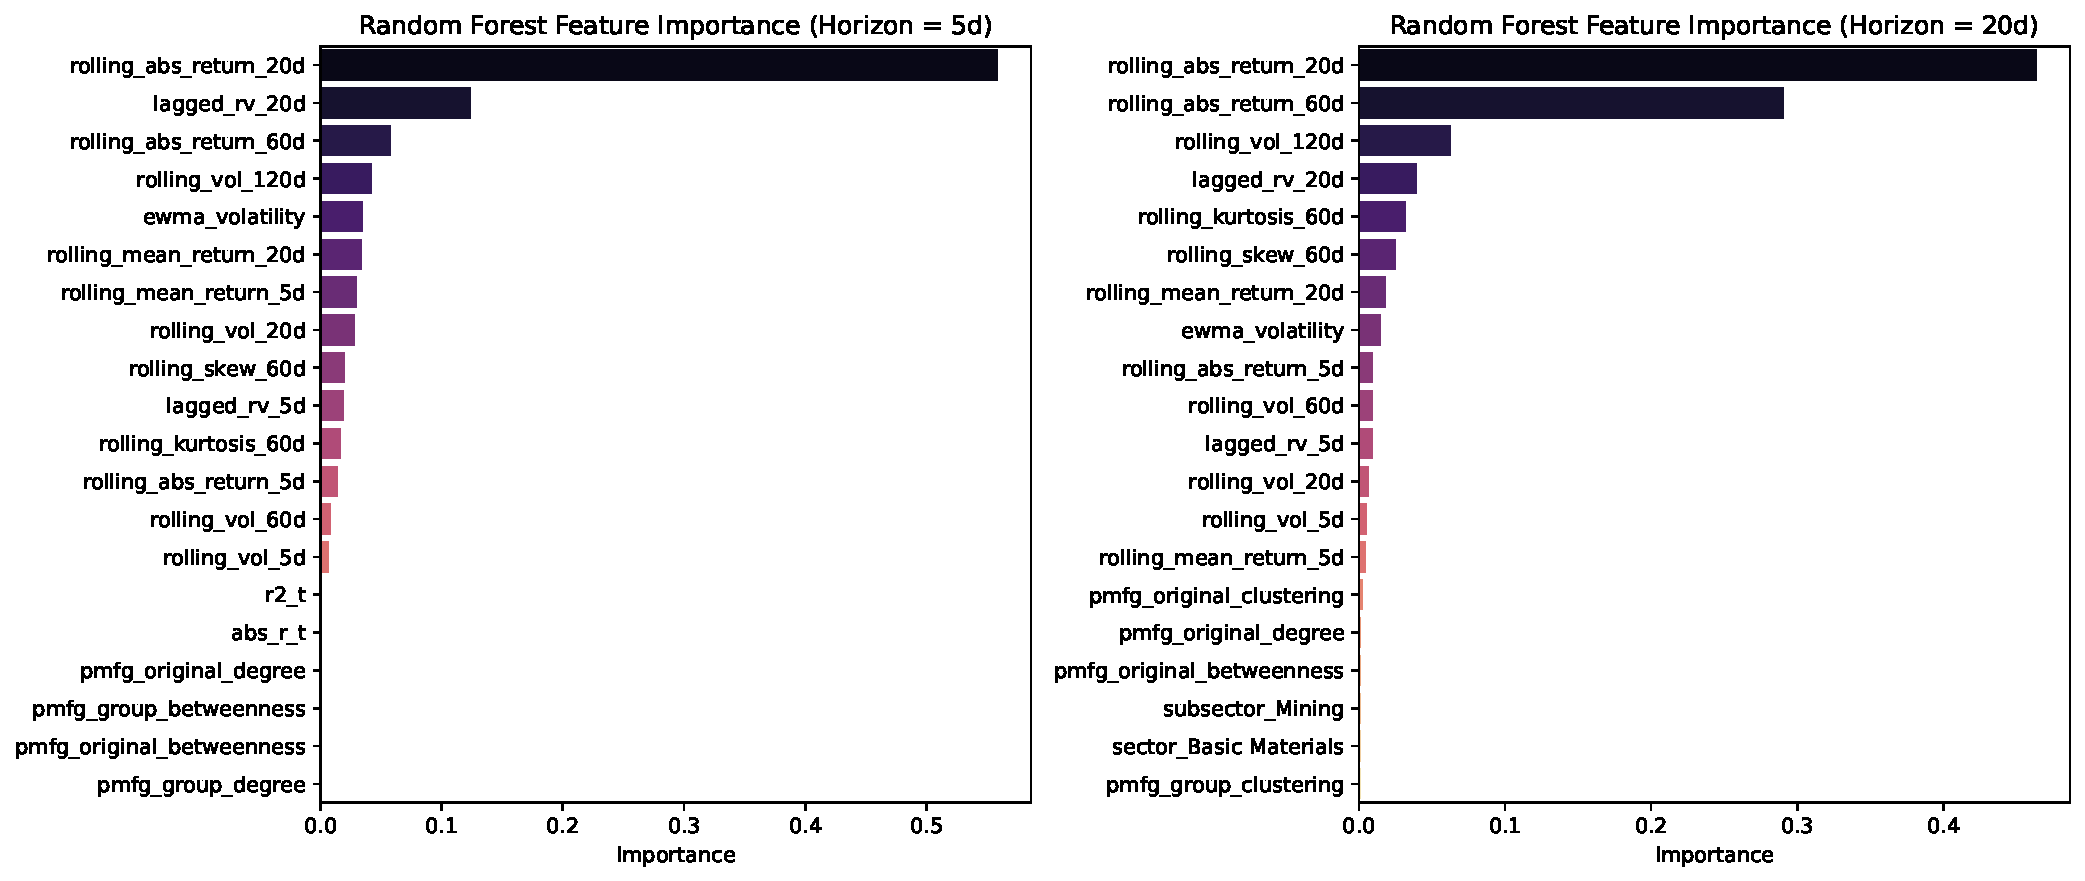
\includegraphics[width=0.95\linewidth]{images/figure_18_ml_feature_importance.pdf}
\caption{Feature importance for Random Forest volatility forecasting models. Classical volatility features dominate, while PMFG and MST variables have smaller but nonzero importance in the network-augmented feature set.}
\label{fig:feature_importance}
\end{figure}
\FloatBarrier

The strongest features are rolling absolute return over 20 days, lagged realized volatility and longer rolling volatility measures. Network features are much smaller, but they are not zero. PMFG clustering, PMFG degree and PMFG betweenness appear among the nonzero network predictors, especially at the 20-day horizon. The appropriate conclusion is therefore incremental: topology does not replace classical volatility features, but it may add structural information when included in a broader feature set.
